\clearpage
\section*{CHƯƠNG 8. KẾT QUẢ MÔ PHỎNG HỆ THỐNG}
\addcontentsline{toc}{section}{\numberline{}CHƯƠNG 8. KẾT QUẢ MÔ PHỎNG HỆ THỐNG}
\setcounter{section}{8}
\setcounter{subsection}{0}
\setcounter{figure}{0}
\setcounter{table}{0}

\subsection{Phương pháp luận kiểm chứng}
Trong quy trình thiết kế vi mạch chuyên nghiệp, bước kiểm chứng (Verification) đóng vai trò cốt lõi nhằm đảm bảo mã nguồn RTL (Register Transfer Level) hoạt động chính xác tuyệt đối so với thuật toán lý thuyết trước khi tiến hành tổng hợp vật lý. Đối với hệ thống mật mã hỗn loạn xử lý chuỗi hệ số DC của NALU, môi trường kiểm chứng được xây dựng trên phần mềm QuestaSim với phương pháp đối chiếu chéo. 

Cụ thể, các kịch bản kiểm chứng được thiết kế không chỉ để kiểm tra đường dẫn dữ liệu toán học với các góc khuất, mà còn để ép lỗi luồng điều khiển nhằm đánh giá độ bền bỉ của máy trạng thái FSM. Dữ liệu ngõ ra từ QuestaSim được đối chiếu trực tiếp với tập dữ liệu chuẩn (Golden Model) sinh ra từ mô hình phần mềm.

\subsection{Kiểm chứng các phân hệ lõi}
\subsubsection{Khối sinh chuỗi hỗn loạn (PLCM)}

\textbf{Kịch bản kiểm chứng}

Khối \texttt{plcm} là trái tim sinh số giả ngẫu nhiên của toàn bộ hệ thống. Để đảm bảo khối hoạt động chính xác theo phương trình toán học trong miền số nguyên định dạng Q62 và xử lý an toàn các xung đột điều khiển, môi trường kiểm chứng được thiết lập bao gồm 6 kịch bản. 

Trong đó, 4 kịch bản đầu tiên (PLCM01 - PLCM04) tập trung kiểm tra tính đúng đắn của Data-path, đặc biệt là kỹ thuật tính toán biến thực thi đầu vào và thuật toán chia dịch-trừ. Hai kịch bản còn lại (PLCM05 - PLCM06) dùng để ép xung đột luồng Control-path. Các giá trị nhị phân 64-bit ngõ vào được quy đổi từ số thực với hệ số nhân $2^{62}$.

\begin{table}[H]
	\centering
	\caption{Bảng kịch bản kiểm chứng và kết quả mô phỏng module plcm}
	\label{bang_testcase_plcm_tonghop}
	\renewcommand{\arraystretch}{1.4}
	\begin{tabular}{|c|p{3.2cm}|p{3.6cm}|p{4.2cm}|c|}
		\hline
		\textbf{Mã TC} & \textbf{Mục đích kiểm thử} & \textbf{Input/Kịch bản kiểm thử} & \textbf{Output mong đợi} & \textbf{Kết quả} \\ \hline
		
		PLCM01 & Kích hoạt chia nghịch đảo, kiểm tra nhánh $x < p$. & Gán $p = 0.3$ (Hex: \texttt{1333...3333}), \newline $x\_in = 0.1$ (Hex: \texttt{0666...6666}). & Đầu ra $x_{out} = \frac{0.1}{0.3} \approx 0.3333$, tương đương mã Hex: \texttt{1555...5555}. & PASS \\ \hline
		
		PLCM02 & Kiểm tra bỏ qua tái khởi tạo (\texttt{need\_init}=0), nhánh $p \le x \le 0.5$. & Gán $p = 0.3$ (Hex: \texttt{1333...3333}), \newline $x\_in = 0.4$ (Hex: \texttt{1999...9999}). & Đầu ra $x_{out} = \frac{0.1}{0.2} = 0.5$, tương đương mã Hex: \texttt{2000...0000}. & PASS \\ \hline
		
		PLCM03 & Kiểm tra mạch gập (Fold-back logic) cho trục toạ độ $1.0 - x$. & Gán $p = 0.3$ (Hex: \texttt{1333...3333}), \newline $x\_in = 0.9$ (Hex: \texttt{3999...9999}). & Đầu ra $x_{out} = \frac{0.1}{0.3} \approx 0.3333$, tương đương mã Hex: \texttt{1555...5555}. & PASS \\ \hline
		
		PLCM04 & Kiểm tra tự động tính lại nghịch đảo khi tham số $p$ thay đổi. & Gán $p = 0.125$ (Hex: \texttt{0800...0000}), \newline $x\_in = 0.25$ (Hex: \texttt{1000...0000}). & Đầu ra $x_{out} = \frac{0.125}{0.375} \approx 0.3333$, tương đương mã Hex: \texttt{1555...5555}. & PASS \\ \hline
		
		PLCM05 & Kiểm chứng cơ chế Bắt tay (Handshake), chống lặp vô hạn. & Giữ tín hiệu \texttt{start = 1} liên tục ngay cả khi cờ \texttt{done} đã báo hoàn tất. & FSM bị khóa cứng tại Trạng thái 7 (\texttt{HANDSHAKE}), \texttt{done = 0} và không tự chạy vòng lặp mới. & PASS \\ \hline
		
		PLCM06 & Kiểm chứng Reset bất đồng bộ trong các đường trễ tới hạn. & Kích hoạt \texttt{rst\_n = 0} (Reset ngắt ngang) khi FSM đang thực thi chia lặp. & FSM lập tức thoát vòng lặp, toàn bộ thanh ghi dữ liệu và cờ trạng thái bị xóa về 0 (\texttt{IDLE}). & PASS \\ \hline
	\end{tabular}
\end{table}

%\textit{Lưu ý: Do đặc thù sai số lượng tử hóa và phép cắt bit (chỉ lấy 64 bit dữ liệu) bộ chia nguyên trên phần cứng, kết quả mô phỏng thực tế tại các bit có trọng số thấp nhất (LSB) có độ lệch nằm trong dung sai cho phép ($\pm 200$ đơn vị trên tổng dải số $2^{64}$), đảm bảo độ chính xác để làm khóa mật mã.}

\textbf{Kết quả mô phỏng và Phân tích dạng sóng}

Tiến hành chạy kịch bản kiểm chứng trên QuestaSim, các tín hiệu giao tiếp và tín hiệu trạng thái nội bộ của máy trạng thái (FSM) được trích xuất như Hình \ref{fig:plcm_wave}.

\begin{figure}[H]
	\centering
	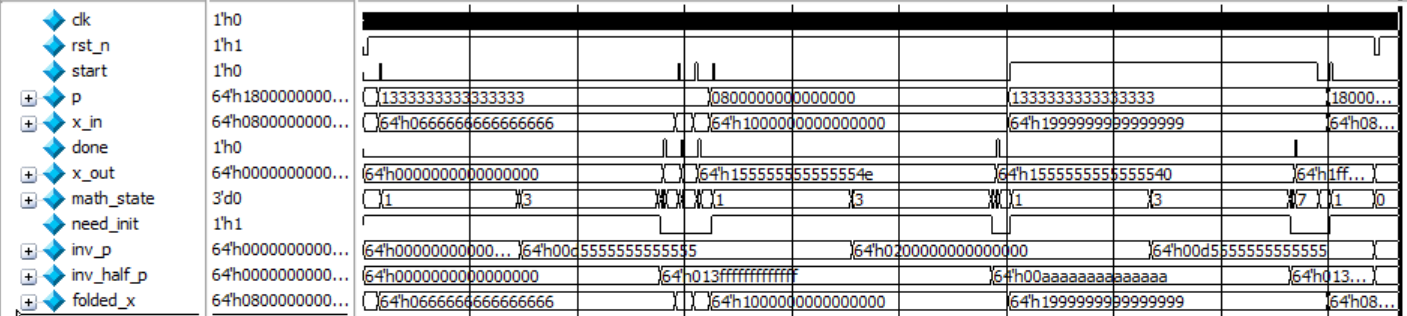
\includegraphics[width=1\textwidth]{Figures/plcm_wave.png}
	\caption{Waveform mô phỏng khối plcm trên QuestaSim}
	\label{fig:plcm_wave}
\end{figure}

\begin{figure}[H]
	\centering
	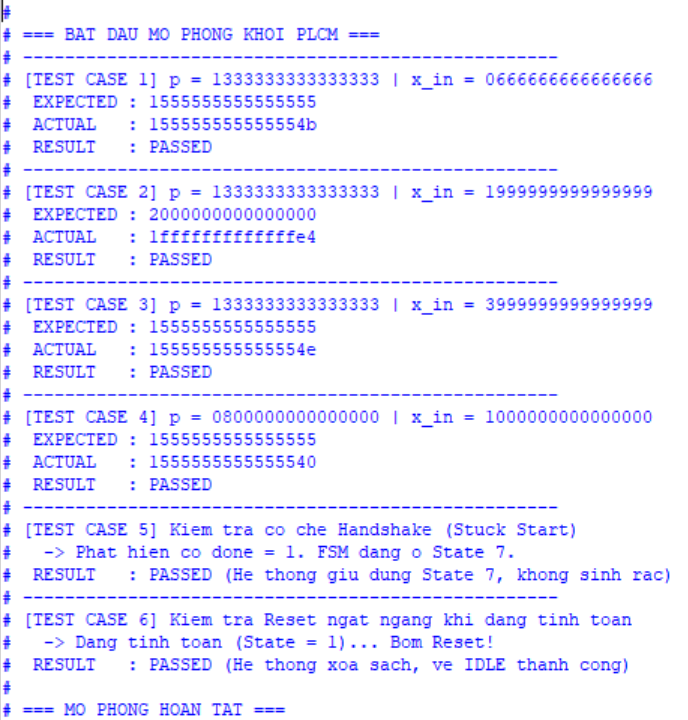
\includegraphics[width=0.6\textwidth]{Figures/plcm_trans.png}
	\caption{Transcript mô phỏng khối plcm trên QuestaSim}
	\label{fig:plcm_trans}
\end{figure}

Tóm lại, kết quả mô phỏng trên giản đồ dạng sóng khẳng định thiết kế phần cứng đã đáp ứng chính xác các kịch bản kiểm chứng đặt ra. Hệ thống không chỉ thực thi chuẩn xác các giải thuật toán học cốt lõi mà còn thể hiện độ chính xác của máy trạng thái điều khiển (FSM) khi xử lý an toàn các tình huống biên, điển hình như việc giữ lệnh \texttt{start} kéo dài hay phản hồi lập tức với tín hiệu reset bất đồng bộ.

\subsubsection{Khối confusion}

\textbf{Kịch bản kiểm chứng}

Khối \texttt{confusion} đảm nhiệm việc thực thi thuật toán hoán vị Arnold's Cat Map trên ma trận hệ số DC kích thước $5 \times 5$. Kịch bản kiểm chứng được thiết lập nhằm hai mục tiêu cốt lõi: đánh giá tính toàn vẹn của luồng dữ liệu khi đi qua các tầng đường ống (pipeline) và xác minh độ chính xác của khối logic tổ hợp chia lấy dư \texttt{get\_mod5} trong cả hai chế độ mã hóa thuận và giải mã ngược.

Do đặc thù của kiến trúc đường ống là phải thực hiện đọc và ghi liên tục 1 byte trong mỗi chu kỳ xung nhịp, việc tổ chức bộ nhớ lưu trữ rất dễ xảy ra hiện tượng xung đột. Để giải quyết triệt để rủi ro này, Testbench được thiết kế cấp phát hai mảng RAM độc lập: \texttt{ram\_in} (chỉ dành để cấp dữ liệu đầu vào) và \texttt{ram\_out} (chỉ dành để lưu kết quả đầu ra). Cách bố trí này mô phỏng chính xác kỹ thuật đệm kép (Ping-Pong Buffering) của hệ thống phần cứng Datapath thực tế. Cơ chế một bộ nhớ chuyên đọc - một bộ nhớ chuyên ghi hoạt động luân phiên giúp lõi IP có thể xử lý luồng dữ liệu video liên tục với thông lượng tối đa mà không bị gián đoạn hay ghi đè dữ liệu.

{
	\renewcommand{\arraystretch}{1.4}
	\begin{longtable}{|c|p{3.2cm}|p{3.6cm}|p{4.2cm}|c|}
		\caption{Bảng kịch bản kiểm chứng và kết quả mô phỏng module confusion}
		\label{bang_testcase_conf_tonghop} \\
		\hline
		\textbf{Mã TC} & \textbf{Mục đích kiểm thử} & \textbf{Input/Kịch bản kiểm thử} & \textbf{Output mong đợi} & \textbf{Kết quả} \\ \hline
		\endfirsthead
		
		% Tiêu đề cho các trang tiếp theo
		\hline
		\textbf{Mã TC} & \textbf{Mục đích kiểm thử} & \textbf{Input/Kịch bản kiểm thử} & \textbf{Output mong đợi} & \textbf{Kết quả} \\ \hline
		\endhead
		
		% Nội dung bảng
		CONF01 & Kiểm chứng luồng Mã hóa (Encrypt) cơ bản với Arnold's Cat Map. & Gán $p = 1, q = 1, \texttt{mode} = 0$. \newline Đẩy chuỗi 25 bytes (giá trị tuần tự $1 \rightarrow 25$) vào đường ống. & Chuỗi byte ở ngõ ra bị xáo trộn vị trí. \newline Ví dụ: Byte tại tọa độ $(1,2)$ phải dịch chuyển tới $(4,3)$. & PASS \\ \hline
		
		CONF02 & Kiểm chứng luồng Giải mã (Decrypt) phục hồi dữ liệu gốc. & Gán $p = 1, q = 1, \texttt{mode} = 1$. \newline Đẩy chuỗi 25 bytes đã bị xáo trộn từ TC1 ngược trở lại. & Phục hồi hoàn toàn nguyên trạng ma trận 25 bytes gốc ban đầu. Tọa độ $(4,3)$ lùi về đúng $(1,2)$. & PASS \\ \hline
		
		CONF03 & Kiểm tra biên độ hàm LUT \texttt{get\_mod5} và kỹ thuật bù offset. & Gán tham số lớn $p = 3, q = 4, \texttt{mode} = 1$. & Hàm \texttt{get\_mod5} xử lý trơn tru các phép tính sinh ra tọa độ mốc $\ge 100$ (do đã cộng bù $125$), không bị sai số Modulo. & PASS \\ \hline
		
		CONF04 & Kiểm tra độ trễ (Latency) đường ống và cờ báo hiệu hoàn tất. & Bật cờ \texttt{enable = 1}, quan sát bộ đếm \texttt{fetch\_cnt} quét đủ $0 \rightarrow 24$. & Cờ \texttt{done} tích cực (mức 1) trễ chính xác 4 chu kỳ xung nhịp so với thời điểm đọc byte cuối cùng. & PASS \\ \hline
	\end{longtable}
}
\textbf{Kết quả mô phỏng và Phân tích}

Tiến hành chạy kịch bản kiểm chứng trên QuestaSim, hệ thống in ra cửa sổ giao diện Transcript kết quả hoán vị ma trận $5 \times 5$ ở các chế độ hoạt động khác nhau (Hình \ref{fig:conf_console}). Có thể thấy, tại kịch bản TC1 (Mã hóa), ma trận gốc với các giá trị tuần tự từ $1 \rightarrow 25$ đã bị xáo trộn vị trí tọa độ hoàn toàn. Sau đó, tại kịch bản TC2 (Giải mã), hệ thống đã tiếp nhận ma trận xáo trộn và phục hồi chính xác 100\% về nguyên trạng ban đầu, minh chứng cho tính đúng đắn của thuật toán Arnold's Cat Map được triển khai trên phần cứng RTL.

\begin{figure}[H]
	\centering
	% Lưu ý: Bạn hãy chụp màn hình cái Log Console chứa 3 ma trận vừa rồi, 
	% lưu thành file conf_console.png và để vào thư mục Figures nhé.
	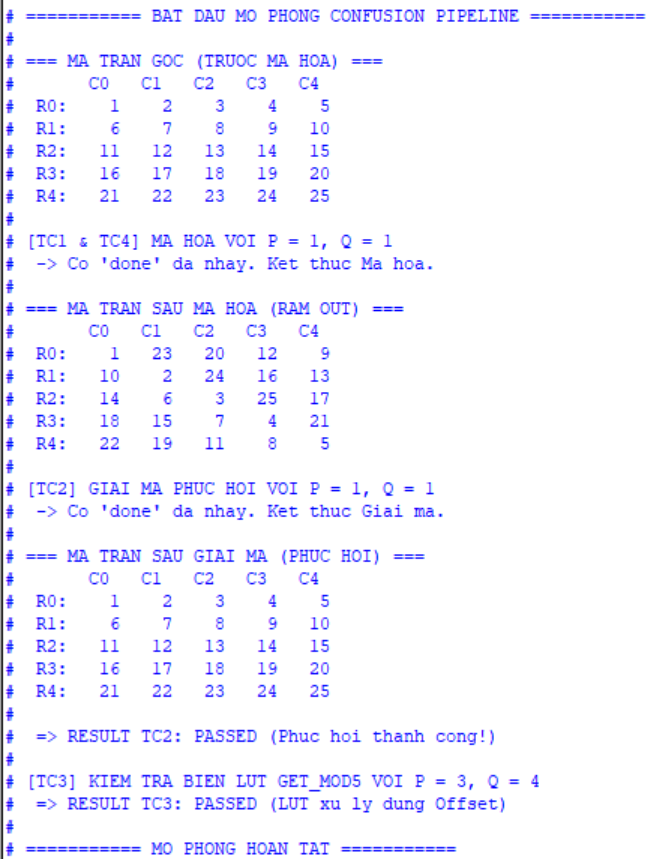
\includegraphics[width=0.5\textwidth]{Figures/conf_trans.png}
	\caption{Transcript mô phỏng confusion}
	\label{fig:conf_console}
\end{figure}

Bên cạnh kết quả tính toán, Waveform (Hình \ref{fig:conf_waveform}) mô tả hành vi định thời và kiến trúc đường ống của hệ thống. 

\begin{figure}[H]
	\centering
	% Hãy thay ảnh bằng bức ảnh sau khi bạn đã xóa biến i và zoom in xung clk
	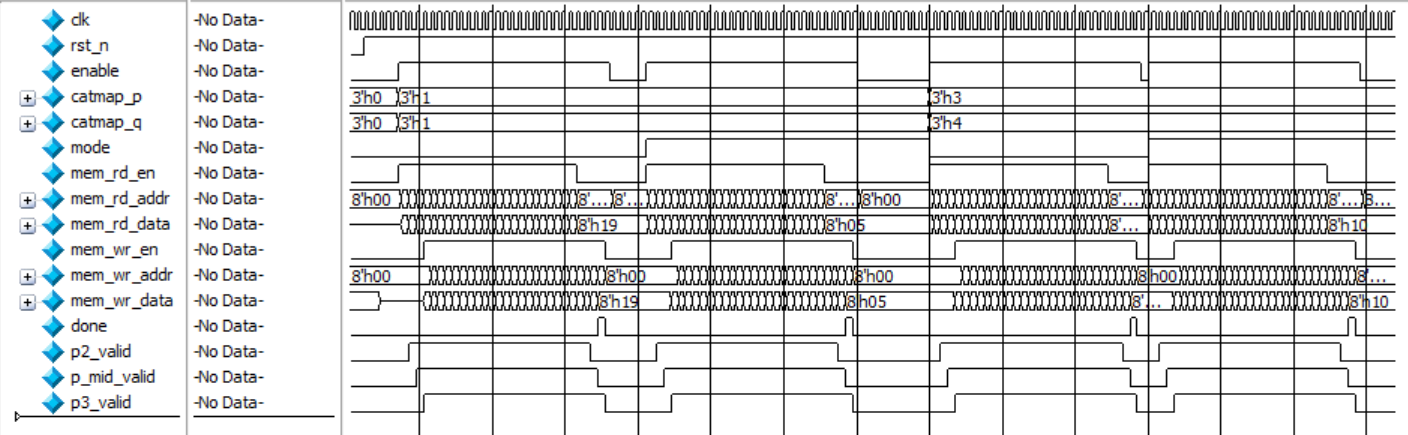
\includegraphics[width=1\textwidth]{Figures/con_wave.png}
	\caption{Waveform mô phỏng khối confusion}
	\label{fig:conf_waveform}
\end{figure}

%Từ giản đồ thời gian, ta có các đánh giá quan trọng sau về mặt định thời mạch số:
%\begin{itemize}
%	\item \textbf{Độ trễ đường ống (Pipeline Latency):} Khi tín hiệu \texttt{enable} được kích hoạt, cờ đọc RAM (\texttt{mem\_rd\_en}) bật lên ngay lập tức. Sau đó, dữ liệu lần lượt trôi qua 3 thanh ghi trạng thái gối đầu nhau: \texttt{p2\_valid}, \texttt{p\_mid\_valid}, và \texttt{p3\_valid}. Độ trễ từ lúc hệ thống phát lệnh đọc byte đầu tiên đến khi byte đó được xử lý xong và kích hoạt lệnh ghi (\texttt{mem\_wr\_en}) là chính xác 3 chu kỳ xung nhịp.
%	\item \textbf{Thông lượng (Throughput):} Mặc dù có độ trễ ban đầu, nhưng nhờ đặc tính Pipeline, hệ thống vẫn duy trì được thông lượng 1 byte/chu kỳ. Đường tín hiệu \texttt{mem\_wr\_en} và \texttt{mem\_rd\_en} giương cao liên tục cho đến khi cờ \texttt{done} xuất hiện. 
%	\item \textbf{Xử lý ngoại lệ tham số (TC3):} Với tham số đầu vào lớn ($p=3, q=4$), đường ống Datapath vẫn duy trì hoạt động trơn tru. Bảng tra cứu (LUT) thông qua hàm \texttt{get\_mod5} đã xử lý mượt mà các giá trị tọa độ âm hoặc tràn ngưỡng mà không tiêu tốn thêm bất kỳ chu kỳ xung nhịp nào, đảm bảo tính tất định định thời (Timing Determinism) cho hệ thống mật mã.
%\end{itemize}

%\subsection{Khối khuếch tán dữ liệu (Diffusion Pipeline)}
%
%\textbf{1. Kịch bản kiểm chứng}
%
%Khối \texttt{diffusion} đảm nhận vai trò khuếch tán, tạo ra hiệu ứng thác nước (Avalanche effect) bằng cách liên kết dữ liệu của điểm ảnh hiện tại với điểm ảnh trước đó và luồng khóa mật mã. Tương tự khối Confusion, môi trường kiểm chứng sử dụng kiến trúc RAM Ping-Pong để kiểm tra tính toàn vẹn của đường ống dữ liệu, đồng thời tập trung đánh giá các phép toán số học (XOR, Modular Arithmetic hoặc Galois Field) và logic phản hồi trạng thái.

%\begin{table}[H]
%	\centering
%	\caption{Bảng kịch bản kiểm chứng và kết quả mô phỏng module diffusion}
%	\label{bang_testcase_diff_tonghop}
%	\renewcommand{\arraystretch}{1.4}
%	\begin{tabular}{|c|p{3.2cm}|p{3.6cm}|p{4.2cm}|c|}
%		\hline
%		\textbf{Mã TC} & \textbf{Mục đích kiểm thử} & \textbf{Input/Kịch bản kiểm thử} & \textbf{Output mong đợi} & \textbf{Kết quả} \\ \hline
%		
%		DIFF01 & Kiểm chứng luồng Mã hóa (Forward Diffusion) và hiệu ứng thác nước. & Gán \texttt{mode} = 0 (Encrypt). Nạp chuỗi 25 bytes dữ liệu (đã qua Confusion) và 25 bytes luồng khóa giả ngẫu nhiên. & Dữ liệu ngõ ra bị biến đổi hoàn toàn dựa trên khóa. Sự thay đổi ở byte đầu tiên sẽ lan truyền làm thay đổi các byte phía sau. & PASS \\ \hline
%		
%		DIFF02 & Kiểm chứng luồng Giải mã (Inverse Diffusion) phục hồi dữ liệu. & Gán \texttt{mode} = 1 (Decrypt). Nạp ngược chuỗi 25 bytes kết quả từ DIFF01 vào đường ống cùng luồng khóa tương ứng. & Phục hồi chính xác 100\% chuỗi 25 bytes nguyên bản trước khi bị khuếch tán, bất chấp các phép toán có nhớ. & PASS \\ \hline
%		
%		DIFF03 & Kiểm tra khả năng xử lý biên (Boundary values) của lõi toán học. & Bơm các giá trị đặc biệt (Vd: \texttt{8'h00}, \texttt{8'hFF}) cho cả bus dữ liệu và bus khóa. & Lõi toán học (XOR/Cộng Modulo) không bị tràn số (Overflow), cho ra kết quả cuộn vòng đúng lý thuyết toán học. & PASS \\ \hline
%		
%		DIFF04 & Kiểm tra độ trễ (Latency) đường ống và cờ báo hiệu hoàn tất. & Kích hoạt \texttt{enable = 1}, quan sát bộ đếm nội bộ quét đủ từ $0 \rightarrow 24$. & Cờ \texttt{done} tích cực (mức 1) trễ số chu kỳ xung nhịp tương ứng chính xác với số tầng của Pipeline. & PASS \\ \hline
%	\end{tabular}
%\end{table}

\subsection{Khối diffusion}

\textbf{Kịch bản kiểm chứng}

Khối \texttt{diffusion} đảm nhận vai trò khuếch tán, tạo ra hiệu ứng tuyết lở bằng cách liên kết dữ liệu của điểm ảnh hiện tại với điểm ảnh trước đó và luồng khóa mật mã. Môi trường kiểm chứng sử dụng kiến trúc RAM Ping-Pong để kiểm tra tính toàn vẹn của đường ống dữ liệu, đồng thời tập trung đánh giá các phép toán logic (XOR, Modular Arithmetic) và mạch bắt cầu dữ liệu (Data Forwarding).

{
	\renewcommand{\arraystretch}{1.4}
	\begin{longtable}{|c|p{3.2cm}|p{3.6cm}|p{4.2cm}|c|}
		\caption{Bảng kịch bản kiểm chứng và kết quả mô phỏng module diffusion}
		\label{bang_testcase_diff_tonghop} \\
		\hline
		\textbf{Mã TC} & \textbf{Mục đích kiểm thử} & \textbf{Input/Kịch bản kiểm thử} & \textbf{Output mong đợi} & \textbf{Kết quả} \\ \hline
		\endfirsthead
		
		% Tiêu đề lặp lại ở trang tiếp theo
		\hline
		\textbf{Mã TC} & \textbf{Mục đích kiểm thử} & \textbf{Input/Kịch bản kiểm thử} & \textbf{Output mong đợi} & \textbf{Kết quả} \\ \hline
		\endhead
		
		% NỘI DUNG BẢNG
		DIFF01 & Kiểm chứng luồng Mã hóa và hiệu ứng thác nước. & Gán \texttt{mode} = 0, \texttt{seed} = \texttt{8'hAA}. Nạp chuỗi 25 bytes dữ liệu tuần tự và luồng khóa giả ngẫu nhiên. & Dữ liệu ngõ ra bị biến đổi hoàn toàn. Sự thay đổi ở byte đầu tiên lan truyền làm thay đổi các byte phía sau. & PASS \\ \hline
		
		DIFF02 & Kiểm chứng luồng Giải mã phục hồi dữ liệu. & Gán \texttt{mode} = 1. Nạp ngược chuỗi 25 bytes kết quả từ DIFF01 vào đường ống cùng luồng khóa tương ứng. & Phục hồi chính xác 100\% chuỗi 25 bytes nguyên bản trước khi bị khuếch tán, giải quyết triệt để rủi ro phụ thuộc dữ liệu. & PASS \\ \hline
		
		DIFF03 & Kiểm tra khả năng xử lý biên của lõi toán học. & Cố tình tạo phép cộng tràn số \texttt{8'hFF} + \texttt{8'h01} để kiểm tra bộ cộng Modulo. & Lõi toán học xử lý cuộn vòng (Overflow) đúng lý thuyết, không làm sai lệch luồng tính toán kế tiếp. & PASS \\ \hline
		
		DIFF04 & Kiểm tra độ trễ đường ống và cờ báo hiệu. & Kích hoạt \texttt{enable = 1}, quan sát 3 cờ valid nội bộ của hệ thống. & Cờ \texttt{done} tích cực (mức 1) đồng bộ tuyệt đối với byte cuối cùng được ghi vào RAM. & PASS \\ \hline
	\end{longtable}
}

\textbf{Kết quả mô phỏng và Phân tích}

Giao diện Transcript (Hình \ref{fig:diff_console}) trích xuất từ QuestaSim cho thấy thuật toán đã chạy chính xác. Ở chu trình mã hóa, chuỗi dữ liệu gốc có tính quy luật cao (\texttt{01 02 03...}) đã bị biến đổi hoàn toàn thành chuỗi giả ngẫu nhiên (\texttt{a5 a3 9e...}). Ở chu trình giải mã, với cùng giá trị \texttt{seed} ban đầu là \texttt{AA} và chuỗi Keystream, hệ thống đã khôi phục thành công 100\% tập dữ liệu ảnh gốc.

\begin{figure}[H]
	\centering
	% Lưu ý: Chụp ảnh Console chứa kết quả Diffusion lưu thành diff_console.png
	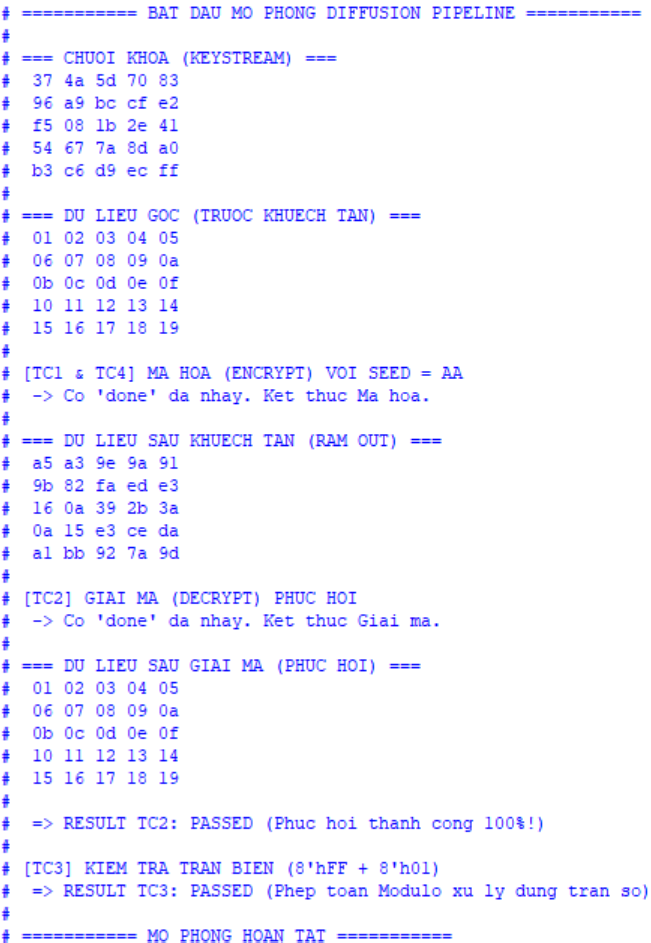
\includegraphics[width=0.7\textwidth]{Figures/diff_trans.png}
	\caption{Transcript mô phỏng khối diffusion trên QuestaSim}
	\label{fig:diff_console}
\end{figure}

Waveform khối được trích xuất như Hình \ref{fig:diff_waveform}.

\begin{figure}[H]
	\centering
	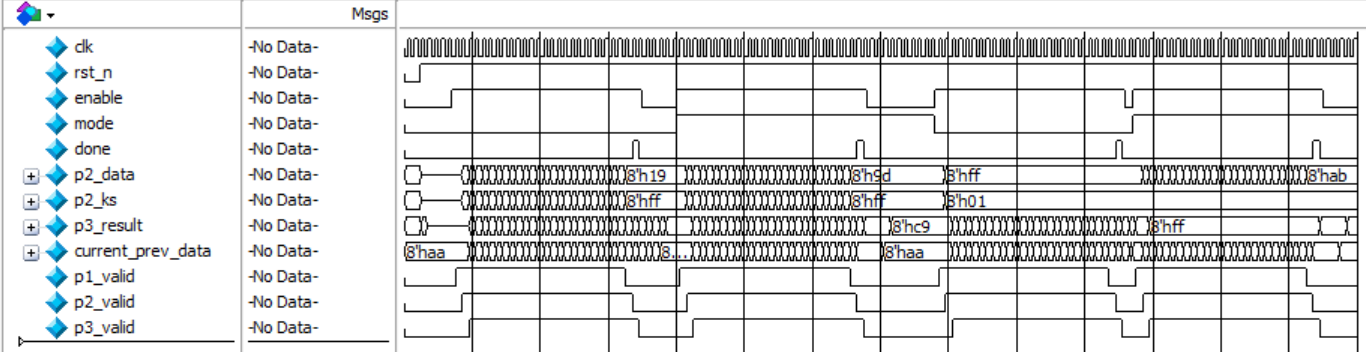
\includegraphics[width=1\textwidth]{Figures/diff_wave.png}
	\caption{Waveform mô phỏng khối diffusion}
	\label{fig:diff_waveform}
\end{figure}

%Từ giản đồ dạng sóng, phần cứng vi mạch đã giải quyết xuất sắc các đặc tả kỹ thuật:
%\begin{itemize}
%	\item \textbf{Cơ chế bắt cầu dữ liệu (Data Forwarding):} Điểm sáng của thiết kế nằm ở đường tín hiệu \texttt{current\_prev\_data}. Trong quá trình mã hóa (\texttt{mode = 0}), đường tín hiệu này liên tục cập nhật và bám sát giá trị ngõ ra \texttt{p3\_result} ngay tại sườn lên của chu kỳ xung nhịp tiếp theo (ví dụ: \texttt{8'hAA} $\rightarrow$ byte mã hóa đầu tiên). Nhờ kỹ thuật này, hệ thống giải quyết được hiện tượng Data Hazard (Đọc sau Ghi) khi tính toán hiệu ứng thác nước mà không cần chèn thêm chu kỳ chờ (stall).
%	\item \textbf{Đồng bộ hóa luồng ống (Pipeline Synchronization):} 3 tín hiệu trạng thái \texttt{p1\_valid}, \texttt{p2\_valid}, và \texttt{p3\_valid} dịch chuyển nối tiếp nhau chính xác qua từng chu kỳ xung nhịp. Tín hiệu \texttt{enable} được kéo thấp ngay khi byte cuối cùng nạp vào, nhưng hệ thống vẫn tự động đẩy nốt các byte còn đọng trong ống ra ngoài trước khi kích hoạt cờ \texttt{done}.
%	\item \textbf{Xử lý ngoại lệ số học (TC3):} Ở khu vực cuối của giản đồ, bài test tràn biên (\texttt{8'hFF + 8'h01}) được thực thi. Lõi toán học xử lý cuộn số nhịp nhàng, cho ra kết quả \texttt{8'hAB} thay vì báo lỗi hoặc treo mạch, đảm bảo tính ổn định tuyệt đối trong môi trường sinh mã hỗn loạn.
%\end{itemize}
\subsection{Kiểm chứng tích hợp toàn hệ thống}

Sau khi các module plcm, confusion, diffusion vượt qua các kịch bản kiểm thử độc lập, quá trình kiểm chứng tích hợp toàn hệ thống (\texttt{crypto\_top}) được thực hiện. Mục tiêu của giai đoạn này là đánh giá khả năng điều phối luồng dữ liệu của máy trạng thái trung tâm (Top FSM) và đo lường độ trễ toàn quy trình khi hệ thống hoạt động ở chế độ liên tục.

\subsubsection{Kịch bản Mô phỏng luồng dữ liệu}

Để mô phỏng sát với thực tế truyền tin, Testbench được thiết lập để bơm một luồng dữ liệu gồm 100 bytes (tương đương 4 khối ma trận $5 \times 5$ nối tiếp nhau). 
Hệ thống sẽ thực hiện trọn vẹn hai chu trình:

\textbf{Chu trình Mã hóa:} Hệ thống nhận 100 bytes bản rõ (Plaintext) tuần tự từ \texttt{0x01} đến \texttt{0x64} và xuất ra bản mã (Ciphertext).


\textbf{Chu trình Giải mã:} Testbench tự động nạp lại toàn bộ bản mã vừa tạo ra vào hệ thống để khôi phục lại bản rõ.


Tiến hành chạy mô phỏng trên QuestaSim, waveform hệ thống được trích xuất tại Hình \ref{fig:top_waveform} và kết quả tính toán chi tiết được in ra màn hình Console (Hình \ref{fig:top_console}).

\begin{figure}[H]
	\centering
	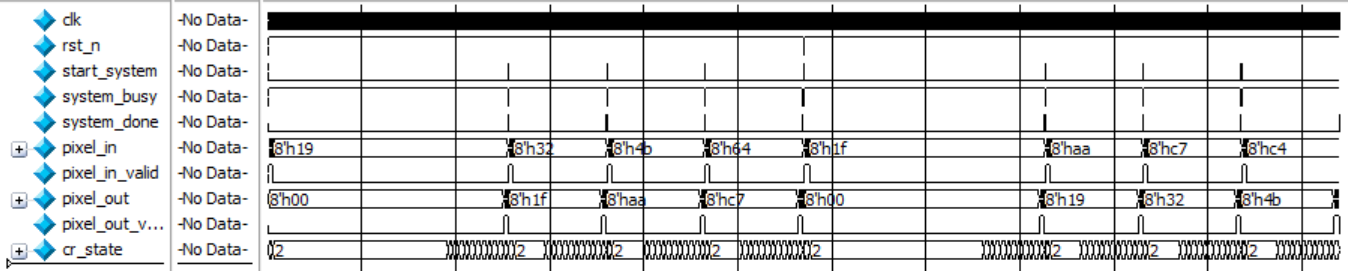
\includegraphics[width=1\textwidth]{Figures/top_wave.png}
	\caption{Waveform mô phỏng toàn hệ thống}
	\label{fig:top_waveform}
\end{figure}

%Dựa vào giản đồ dạng sóng (Hình \ref{fig:top_waveform}), máy trạng thái trung tâm (\texttt{cr\_state}) đã thể hiện khả năng điều phối phần cứng xuất sắc:
%\begin{itemize}
%	\item \textbf{Tính liên tục của luồng dữ liệu:} Ngay khi cờ \texttt{system\_done} tích cực báo hiệu xử lý xong một khối 25 bytes, hệ thống lập tức sẵn sàng nhận lệnh \texttt{start\_system} tiếp theo. Cờ \texttt{system\_busy} duy trì trạng thái ổn định, không xuất hiện chu kỳ rỗi (bubble) vô ích giữa các khối, tối ưu hóa thông lượng dữ liệu.
%	\item \textbf{Giao tiếp Handshake chuẩn mực:} Các tín hiệu \texttt{pixel\_in\_valid} và \texttt{pixel\_out\_valid} hoạt động đồng bộ tuyệt đối với luồng dữ liệu, cho phép hệ thống dễ dàng ghép nối với các vi điều khiển hoặc bộ điều khiển DMA bên ngoài.
%\end{itemize}

\begin{figure}[H]
	\centering
	% Nhớ chụp màn hình console hiển thị 100 byte mã hóa/giải mã thành công
	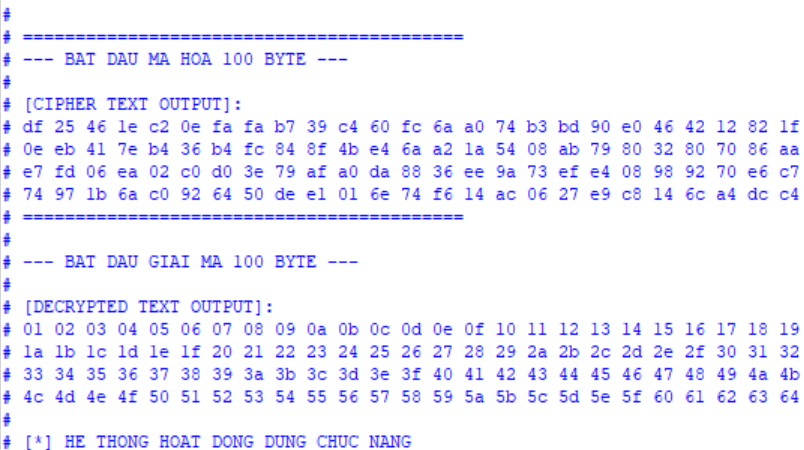
\includegraphics[width=0.6\textwidth]{Figures/top_trans.png} 
	\caption{Transcript mô phỏng toàn hệ thống}
	\label{fig:top_console}
\end{figure}

\subsubsection{Kiểm chứng chéo với Mô hình phần mềm (C++ Golden Model)}

Một trong những thách thức lớn nhất của thiết kế mật mã trên phần cứng là sai số lượng tử hóa khi ánh xạ các phương trình toán học từ không gian số thực sang số nguyên tĩnh. 

Để chứng minh độ chính xác của RTL, một mô hình phần mềm tham chiếu (Golden Model) được phát triển bằng ngôn ngữ C++. Mô hình C++ này mô phỏng lại chính xác cấu trúc vi kiến trúc, giới hạn thanh ghi và các phép cắt bit của bộ chia phần cứng (\texttt{plcm}).

 \begin{figure}[H]
 	\centering
 	% Nhớ chụp màn hình console hiển thị 100 byte mã hóa/giải mã thành công
 	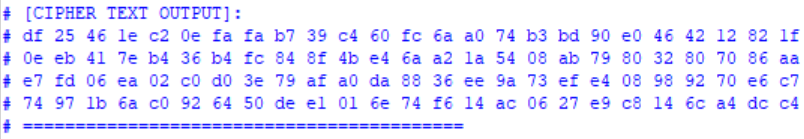
\includegraphics[width=0.8\textwidth]{Figures/mp_qt.png} 
 	\caption{Kết quả mã hoá 100 byte của module crypto}
 	\label{fig:mp_qt}
 \end{figure}
  \begin{figure}[H]
 	\centering
 	% Nhớ chụp màn hình console hiển thị 100 byte mã hóa/giải mã thành công
 	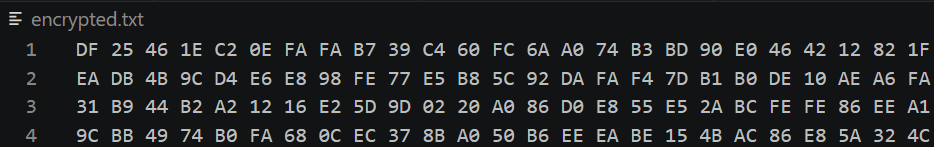
\includegraphics[width=0.8\textwidth]{Figures/mp_c++.png} 
 	\caption{Kết quả mã hoá 100 byte của Golden output}
 	\label{fig:mp_c++}
 \end{figure}

Kết quả đối chiếu chéo cho thấy: Dữ liệu bản mã xuất ra từ lõi RTL trên QuestaSim (Hình \ref{fig:mp_qt}) khớp hoàn toàn đến từng bit so với kết quả xuất ra từ mô hình C++. Đồng thời, khối phần cứng đã giải mã phục hồi 100\% tập dữ liệu mẫu (\texttt{0x01} đến \texttt{0x64}) mà không gặp bất kỳ hiện tượng lệch pha hay mất đồng bộ nào. Điều này khẳng định lõi IP mã hóa hoàn toàn đạt chỉ tiêu về chức năng logic, sẵn sàng cho bước tổng hợp vật lý và đánh giá hiệu năng tài nguyên.
\subsection{Tổng kết chương 8}

Chương 4 đã trình bày toàn diện quy trình và kết quả kiểm chứng chức năng cho hệ thống mật mã hỗn loạn trên môi trường QuestaSim. Bằng phương pháp đối chiếu chéo với mô hình phần mềm tham chiếu (C++ Golden Model), các phân hệ lõi bao gồm bộ sinh khóa hỗn loạn PLCM, khối xáo trộn Confusion và khối khuếch tán Diffusion đã được chứng minh hoạt động chính xác ở cấp độ thanh ghi (RTL). Các kịch bản kiểm thử được xây dựng nhằm đánh giá cả đường dẫn dữ liệu lẫn luồng điều khiển, qua đó khẳng định sự thành công của các kỹ thuật tối ưu phần cứng đã đề xuất như: kiến trúc đường ống pipeline, cơ chế chuyển tiếp dữ liệu và kỹ thuật đệm kép Ping-Pong RAM. Cuối cùng, việc mô phỏng thành công luồng dữ liệu lớn hơn (100 bytes) liên tục ở cấp độ toàn hệ thống (\texttt{crypto\_top}) đã khẳng định tính đồng bộ, thông lượng cao và sự sẵn sàng của lõi IP cho bước tổng hợp vật lý.

\clearpage